\documentclass{beamer}
\usetheme{Copenhagen}
\usepackage{polyglossia}
\usepackage{tabu}
\usepackage{multicol}


\usepackage{tikz}
\usetikzlibrary{matrix}
\usepackage{tkz-berge}
\usetikzlibrary{shapes,snakes,mindmap}
\definecolor{lightblue}{RGB}{160,180,200}
\definecolor{darkblue}{RGB}{110,130,150}
\definecolor{lightred}{RGB}{200,10,10}
\setdefaultlanguage{english}


\title{So you're a Linux kernel developer? \\Name all subsytems.}
%\subtitle{Name all subsystems.}

%\usetheme{lucid}
\begin{document}
	\frame {
		\titlepage
		\includegraphics[scale=0.25]{OTH_LOGO.png}
	}

	%\begin{frame}
	%\frametitle{Topics}
	%	\begin{block}{}

	%	\end{block}
	%\end{frame}

	%TODO: TIKZ-Diagramm um Section Graph zu verdeutlichen, vllt noch Files reinmachen
	%TODO: Coole Trivia zu neuen Subsystemen einholen, damit man mehr darüber reden kann
	%TODO: Fragestellungen, die man beantworten möchte/Probleme, die man lösen möchte
	%TODO: alle Kontributoren, Collaboration mit der Uni Passau, dass alles, was wir machen, auch Anwendung hat und der Community was bringen soll, Elisa erwähnen

	%Thank you very much
	%isn't much to say about me
	%which is what my bachelor thesis is about

	\begin{frame}
	\frametitle{Speaker Introduction}
	\begin{columns}
		\begin{column}{0.65\textwidth}
			\begin{block}{Pia Eichinger}
			\begin{itemize}
			\item Student at the University of Applied Sciences in Regensburg (OTH Regensburg)
			\item pia.eichinger@st.oth-regensburg.de
			\item Researched organisational and maintenance structure of the Linux kernel
			\end{itemize}
			\end{block}
		\end{column}
		\begin{column}{0.3\textwidth}
     		\includegraphics[width=1.0\textwidth]{pics/speaker_piaei.jpg}
		\end{column}
	\end{columns}
	\end{frame}


	\begin{frame}
	\frametitle{Research Group: Co-Authors}
	\begin{minipage}[c]{1.0\linewidth}
		\begin{columns}
		\begin{column}{0.35\textwidth}
			\begin{center}
     		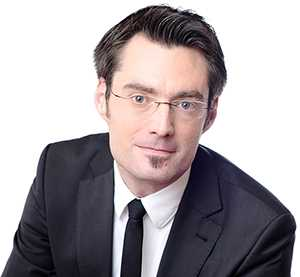
\includegraphics[width=0.5\textwidth]{pics/speakers_mauerer.jpeg}
			\end{center}
		\end{column}
		\begin{column}{0.7\textwidth}
		\begin{block}{Wolfgang Mauerer}
			\begin{itemize}
				\item Professor for theoretical computer science
				\item wolfgang.mauerer@othr.de
			\end{itemize}
		\end{block}
		\end{column}
		\end{columns}

	\end{minipage}
	\begin{minipage}[c]{1.0\linewidth}
		\begin{columns}
		\begin{column}{0.35\textwidth}
			\begin{center}
     		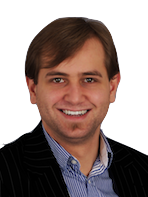
\includegraphics[width=0.5\textwidth]{pics/speakers_ralf.png}
			\end{center}
		\end{column}
		\begin{column}{0.7\textwidth}
		\begin{block}{Ralf Ramsauer}
			\begin{itemize}
				\item PhD student
				\item ralf.ramsauer@othr.de
			\end{itemize}
		\end{block}
			%Ralf Ramsauer\\PhD student \\
		\end{column}
		\end{columns}
	\end{minipage}
	\begin{minipage}[c]{1.0\linewidth}
		\begin{columns}
		\begin{column}{0.35\textwidth}
			\begin{center}
     		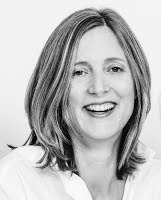
\includegraphics[width=0.5\textwidth]{pics/speakers_scherzinger.jpeg}
			\end{center}
		\end{column}
		\begin{column}{0.7\textwidth}
		\begin{block}{Stefanie Scherzinger}
			\begin{itemize}
				\item Professor for scalable database systems
				\item stefanie.scherzinger@uni-passau.de
			\end{itemize}
		\end{block}
			%Stefanie Scherzinger\\Professor for scalable database systems\\stefanie.scherzinger@uni-passau.de
		\end{column}
		\end{columns}
	\end{minipage}
	\end{frame}


	\begin{frame}
	\frametitle{Collaboration and Motivation}
		\begin{block}{Motivation and Goals}
			\begin{itemize}
				\item Formalising/Assessing the Linux kernel development process
				\item Improve/Quantify the development process
				\item Tools to support the open source community
				\item Safety-Critical Development
			\end{itemize}
		\end{block}
		\begin{block}{Collaboration Partners}
			\begin{itemize}
				\item ELISA
				\item University of Passau
			\end{itemize}
		\end{block}
		$\Rightarrow$ Statistical Methods to research/understand the development process
	\end{frame}

	\begin{frame}
	\frametitle{Bachelor Thesis - Motivation and Beginnings}
		\begin{block}{Linux + Safety Critical Environments}
			= Development Process: Major certification challenges
		\end{block}
		$\Rightarrow$ Ex post facto analysis\\ %TODO: Ex post facto analysis\\
		%\Rightarrow Process characterisation with hindsight
		$\Rightarrow$ Characterize the process with hindsight

		\begin{alertblock}{Goal}
			\begin{itemize}
				\item Analytical quantitative software engineering
				\item Analyse patch integration
			\end{itemize}
			%Use analytical tools for quantitive software engineering to analyse patch integration in the Linux kernel repository. %TODO: Aufspalten Mit analytischem quantitativen Softwareengineering wird des gmacht
		\end{alertblock}
	\end{frame}


	\begin{frame}
	\frametitle{Maintainers Hierarchy}
     		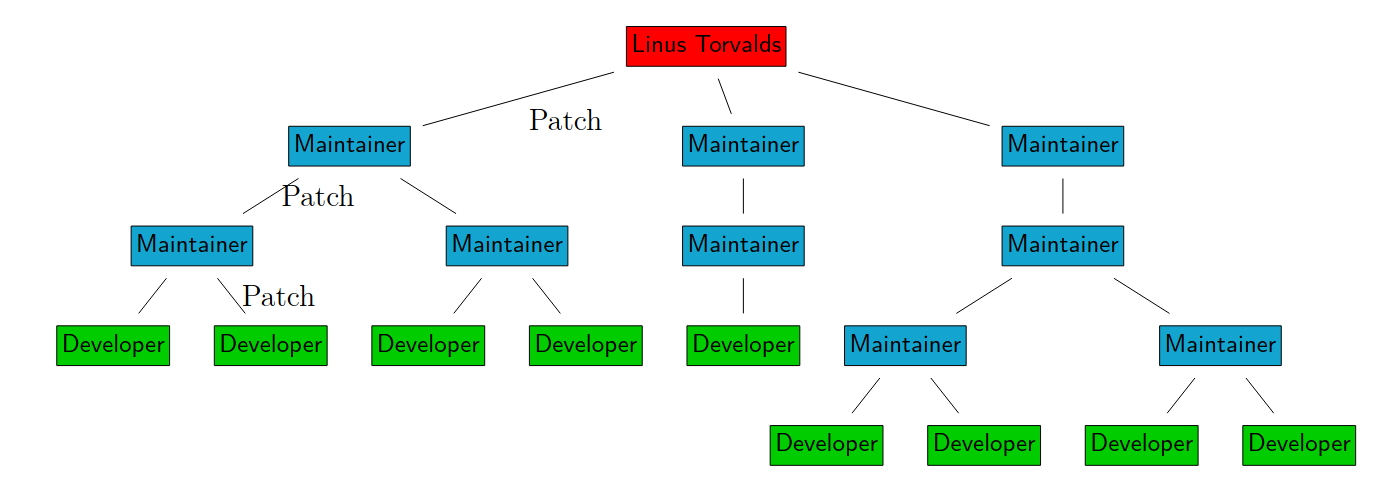
\includegraphics[width=1.0\textwidth]{pics/maintainers_hierarchy.png}
	\end{frame}


	\begin{frame}
	\frametitle{Bachelor Thesis - Motivation and Beginnings}
		\begin{block}{Original Projects}
			\begin{itemize}
				\item Conform Integration of Patches
				\item Patch traversal through MAINTAINERS hierarchy
				%\item How do the different subsystems compare in regards to integration?
			\end{itemize}
		\end{block}
	\end{frame}


	\begin{frame}
	\frametitle{The Subsystem Problem}
		\begin{alertblock}{Only problem is ...}
			\begin{itemize}
				\item \textbf{... where can I find the maintainers hierarchy?}
				\item \textbf{... where can I find the documentation on all subsystems?}
				\item \textbf{... what exactly \textit{is} a subsystem even?}
			\end{itemize}
		\end{alertblock}
	\end{frame}


	\begin{frame}
	\frametitle{The Subsystem Problem - What is a subsystem?}
	%\begin{block}{Documentation: Early-stage Planning in the Linux Kernel Development Process}
	%	"Again, the MAINTAINERS file is	the place to start.  That file tends to not always be up to date, though, and not all \textbf{subsystems} are represented there."

	%	$\Rightarrow$ Every single entry in MAINTAINERS is one subsystem.
	%\end{block}

	%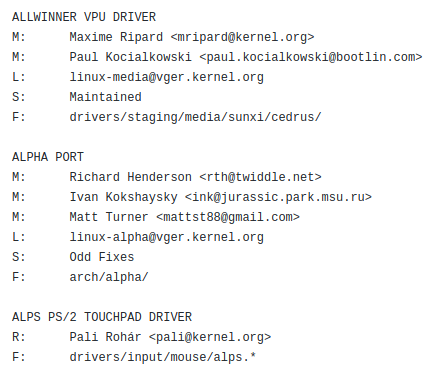
\includegraphics[scale=0.25]{pics/MAINTAINERSbild.png}
	\begin{columns}
		\begin{column}{0.55\textwidth}
			\begin{block}{Docs: Early-stage Planning}
				"Again, the MAINTAINERS file is	the place to start. [...] not all \textbf{subsystems} are represented there."
			\end{block}
			\begin{center}
     		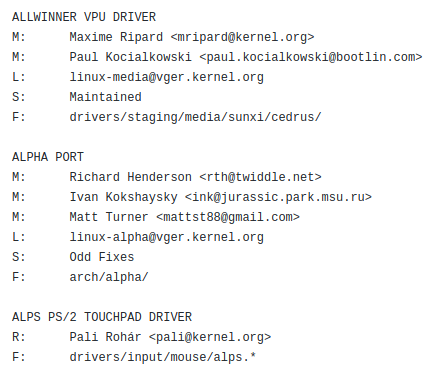
\includegraphics[width=0.6\textwidth]{pics/MAINTAINERSbild.png}
			\end{center}
		\end{column}
		\begin{column}{0.5\textwidth}
			\begin{center}
			$\Rightarrow$ \textbf{Subsystems}
			\end{center}
		\end{column}
	\end{columns}
	\end{frame}


	\begin{frame}
	\frametitle{The Subsystem Problem - What is a subsystem?}
	\begin{center}
     	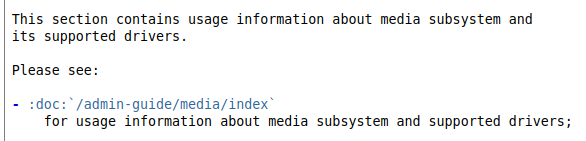
\includegraphics[width=0.6\textwidth]{pics/Media_subsystem.png}
	\end{center}

	\begin{block}{But... }
		\begin{itemize}
		\item No "Media"/"Media Subsystem" entry in MAINTAINERS
		\item Over 100 "subsystems" \textit{containing} the word "Media"
		\end{itemize}
	\end{block}
	\begin{center}
	$\Rightarrow$ Which one?
	\end{center}
	\end{frame}

	\begin{frame} %TODO: Entries in MAINTAINERS: sections, rechts in Bsp veranschaulichen
	\frametitle{Subsystem Definition}
		\begin{block}{Definition: Subsystem}
			Entries in MAINTAINERS: \textbf{sections}

			Sections share files (measured in Lines of Code): \textbf{thematically related}

			Grouping of thematically strong related sections: \textbf{subsystem}.

		\end{block}
	\end{frame}

	\begin{frame}
	\frametitle{Bachelor Thesis - Change of Research Question}
		\begin{block}{No clear listing of subsystems}
			$\Rightarrow$ Let's find out!
		\end{block}

		\begin{block}{Research Projects}
			\begin{itemize}
				\item Conform Integration of Patches
				\item Subsystem Detection
			\end{itemize}
		\end{block}
	\end{frame}


	\begin{frame}
	\frametitle{Definition: Section Graph}
	\begin{alertblock}{Goal: Find and analyse subsystems}
		Visualise MAINTAINERS sections and thematical relations
	\end{alertblock}

		\begin{block}{Definition: Section Graph}
			\begin{itemize}
				\item Undirected Graph
				\item \textit{Vertices}: Sections of MAINTAINERS
				%\item \textit{Vertex Weight}: accumulated LoC of all relevant files for the section
				\item \textit{Edge}: Do two sections share LoC? Yes $\Rightarrow$ Edge
				%\item \textit{Edge Weight}: accumulated LoC of all shared files of both sections
			\end{itemize}
		\end{block}

		$\Rightarrow$ Detect clusters (subsystems)

		%$\Rightarrow$ Find subsystems by finding clusters with common community detection algorithms (Walktrap) %TODO: etablierte Verfahren, referenziere Paper Mitchell Choblins Mauerer, Abels, wir ham Gedanken drüber gmacht, etabliertes Verfahren, wurde damit entwickelt und wir nehmen ned IRGENDWAS
	\end{frame}

\begin{frame}
	\frametitle{Visualisation: Section Graph}
	\begin{columns}
		\begin{column}{0.4\textwidth}
\begin{tikzpicture}
    \begin{scope}[shift={(3cm,-5cm)}, fill opacity=0.5]
        \draw[fill=blue, draw = black] (0,0) circle (2);
        \draw[fill=green, draw = black] (-1.5,0) circle (1);
    \draw[fill=red, draw = black] (1.5,0) circle (1);
    %\node at (0,4) (A) {\large\textbf{A}};
    \node at (-2,1) (B) {\large\textbf{B}};
    \node at (2,1) (C) {\large\textbf{C}};
    \node at (0,0) (A) {\large\textbf{A}};

    \end{scope}

\end{tikzpicture}
		\end{column}
		\begin{column}{0.55\textwidth}
%\begin{tikzpicture}
%\tikzstyle{every node}=[draw, circle, fill=black, inner sep=0pt,minimum size=3pt]
%\draw (0,4) node(6){} -- (2,3) node(5){} -- (2,1) node(4){} -- (0,0) node(3){} -- (-2,1) node(2){} -- (-2,3) node(1){} -- cycle;
%\draw[color=red] (1) -- (3);
%\end{tikzpicture}
\begin{center}
\begin{tikzpicture}
\tikzstyle{every node}=[draw, circle, fill=white, inner sep=0pt,minimum size=3pt]
%\draw[color=green] (2,0) node(4){H4} -- (7,-5) -- (7,-7) -- (6,-8) -- (4,-8) -- (3,-7) -- (3,-6) node(44){H4};
%\draw[color=green] (2,0) node(4){H4} -- (7,-5) node(44){H4};

%\draw[color=red] (0,-5) node (3){H3} -- (12,-5) node (33){H3};
\draw[color=black] (0,0) -- (1,1);
\draw[color=black] (1,1) -- (0,2);
\draw[color=blue] (1, 1) node {A};
\draw[color=green] (0, 0) node {B};
\draw[color=lightred] (0, 2) node {C};
%\draw[color=black] (1,-1) node {B};
%\draw[color=yellow] (0,0) node {A} -- (1,1) node {B};
%\draw[color=orange] (1,1) node (2){H2} -- (1,-1) node (22){H2};
%
%\draw[color=pink] (12,-3) node(5){H5} -- (8,-7) node (5){H5};

\end{tikzpicture}
\end{center}
%\begin{tikzpicture}[concept, outer sep=0pt, color=lightblue, 
%%every node/.style= {circle,fill={lightred},draw=black, line width=1pt,inner sep=2.7pt},
%every node/.style= {circle,draw=black, line width=1pt,inner sep=2.7pt},
%every path/.style={circle connection bar, fill=darkblue}]
%  \SetVertexNoLabel
%  \begin{scope}[xshift=12cm]
%    \grEmptyCycle[RA=2/sin(60)]{3}
%  \end{scope}
%  \AssignVertexLabel{a}{A,B,C}
%  %\VertexLightFillColor{a}{lightblue, green, red}
%  %\VertexFillColor{A}{green}
%  \Edges(a0,a1)
%  \Edges(a0,a2)
%  %\Edges(a4,a0,a3)
%\end{tikzpicture}
		\end{column}
	\end{columns}
\begin{center}


\end{center}
\end{frame}

	\begin{frame}
	\frametitle{Top-20\% Section Graph}
	\begin{center}
	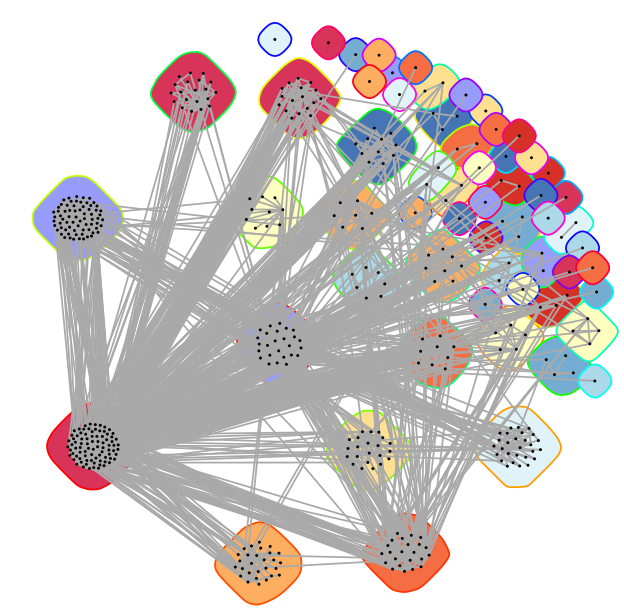
\includegraphics[scale=0.3]{pics/SectionGraph_NoLabels.png}
	\end{center}
	\end{frame}



	\begin{frame}
	\frametitle{Cluster Discussion and Terminology}
		\begin{alertblock}{Cluster Discussion}
			\begin{itemize}
				\item Each major cluster: \textbf{isolated graph}
				\item "Recluster" again from within
			\end{itemize}
		\end{alertblock}
		
		\begin{block}{Terminology}
			\begin{itemize}
				\item Isolated cluster as own graph: \textbf{Cluster Graph}
				\item Cluster found within cluster graph: \textbf{Subcluster}
				%\item Vertex degree within entire section graph: \textbf{Outer Degree}
				%\item Vertex degree within cluster graph: \textbf{Inner Degree}
			\end{itemize}
		\end{block}
	\end{frame}

	\begin{frame}
	\frametitle{Reminder: Research Questions}
		\begin{alertblock}{Conform Patch Integration}
			Patch integrated by relevant maintainer (from MAINTAINERS) $\Rightarrow$ \textbf{Conform Integration}
		\end{alertblock}

		\begin{block}{TL;DR}
			\begin{itemize}
				\item Analyse recent patch integrations
				\item Determine \textit{conform} patch integration
				%\item Research recent patches in mainline and by which maintainer they were originally committed
				%\item Maintainer relevant according to get\_maintainer.pl? $\Rightarrow$ "correctly" integrated
				%\item Research on all major lists with highest patch traffic
				%\item Go into detail as to \textit{why} a maintainer might have "incorrectly" committed patches outside of their relevant subsystem
			\end{itemize}
		\end{block}
		$\Rightarrow$ Analyse reasons for "incorrect" patch integration
	\end{frame}


	\begin{frame}
	\frametitle{Conform Patch Integration}
	\begin{center}
	
\includegraphics[scale=0.05]{pics/exclamation.jpeg}
	\end{center}

		\begin{alertblock}{Important Note}
			\begin{itemize}
				\item We do not mean to point fingers!
				\item Goal: Classify Patch Integration in \textit{some} way
			\end{itemize}
		\end{alertblock}
	\end{frame}

	\begin{frame}
	\frametitle{Future Work}
		\begin{block}{Future Work}
			\begin{itemize}
				\item Combination: Subsystems and Conform Patch Integration
				\item Cluster discussion on full section graph
				\item Visualise earlier versions and development
				\item Apply section graph to other open source projects (QEMU, U-Boot)
				\item Maintainer Graph
			\end{itemize}
		\end{block}

		All work integrated in https://github.com/lfd/PaStA
	\end{frame}

	\begin{frame}
	\frametitle{Research Group}
	\begin{minipage}[c]{1.0\linewidth}
		\begin{columns}
		\begin{column}{0.35\textwidth}
			\begin{center}
     		\includegraphics[width=0.3\textwidth]{pics/speaker_piaei.jpg}
			\end{center}
		\end{column}
		\begin{column}{0.7\textwidth}
		\begin{block}{Pia Eichinger}
			pia.eichinger@st.oth-regensburg.de
		\end{block}
		\end{column}
		\end{columns}

	\end{minipage}
	\begin{minipage}[c]{1.0\linewidth}
		\begin{columns}
		\begin{column}{0.35\textwidth}
			\begin{center}
     		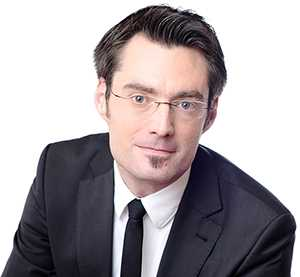
\includegraphics[width=0.3\textwidth]{pics/speakers_mauerer.jpeg}
			\end{center}
		\end{column}
		\begin{column}{0.7\textwidth}
		\begin{block}{Wolfgang Mauerer}
			wolfgang.mauerer@othr.de
		\end{block}
		\end{column}
		\end{columns}

	\end{minipage}
	\begin{minipage}[c]{1.0\linewidth}
		\begin{columns}
		\begin{column}{0.35\textwidth}
			\begin{center}
     		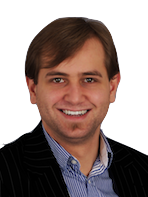
\includegraphics[width=0.3\textwidth]{pics/speakers_ralf.png}
			\end{center}
		\end{column}
		\begin{column}{0.7\textwidth}
		\begin{block}{Ralf Ramsauer}
			ralf.ramsauer@othr.de
		\end{block}
			%Ralf Ramsauer\\PhD student \\
		\end{column}
		\end{columns}
	\end{minipage}
	\begin{minipage}[c]{1.0\linewidth}
		\begin{columns}
		\begin{column}{0.35\textwidth}
			\begin{center}
     		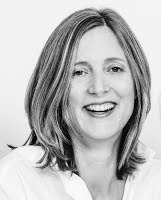
\includegraphics[width=0.3\textwidth]{pics/speakers_scherzinger.jpeg}
			\end{center}
		\end{column}
		\begin{column}{0.7\textwidth}
		\begin{block}{Stefanie Scherzinger}
			stefanie.scherzinger@uni-passau.de
		\end{block}
			%Stefanie Scherzinger\\Professor for scalable database systems\\stefanie.scherzinger@uni-passau.de
		\end{column}
		\end{columns}
	\end{minipage}
	\end{frame}


\end{document}
